\chapter[Conductance in the Mixed-Valence Regime]{Occupation Resolved Conductance in the Mixed-Valence Regime}\label{cha:mixed_valence_conductance}

To my knowledge, the following work in this chapter is the first time that conductance and charge transitions have been simultaneously measured to resolve the conductance enhancement due to the Kondo effect as function of the occupation in an experiment. The conductance enhancement is most pronounced when the quantum dot is strongly coupled ($\mathrm{\Gamma/k_BT}>>1$) to the source and drain leads so it natural to measure the Kondo effect in this regime. However, when the coupling is strong, charge transitions spread out and they become difficult to convert into occupation. The following work falls between the tightly defined window of strong coupling to see the Kondo effect and weak coupling where charge transitions are easily measured. 



\begin{figure}[ht]
  \begin{center}
%% includegraphics: comment the following if not using the graphicx package
    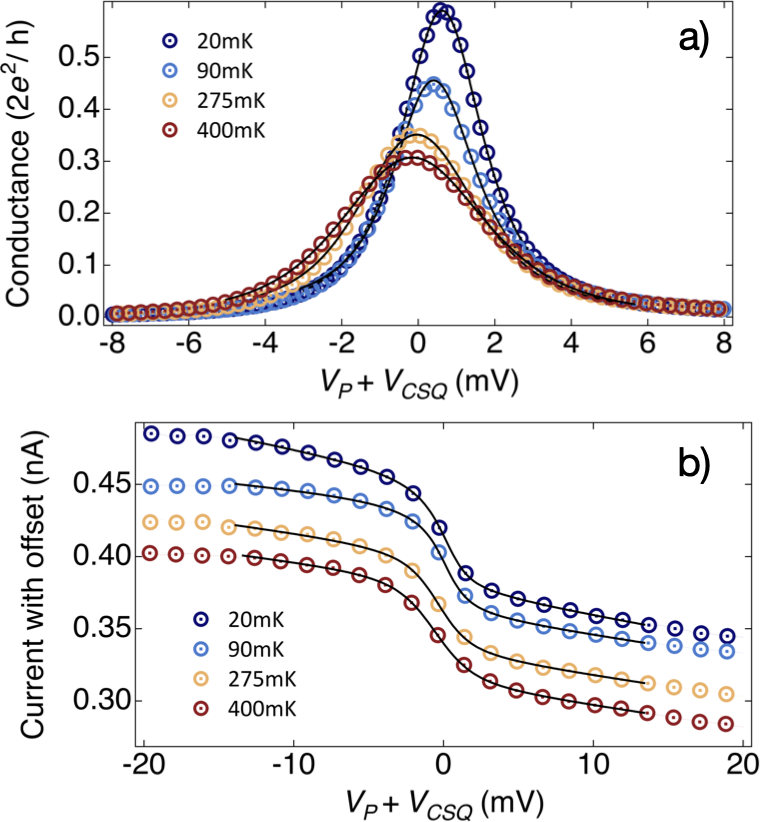
\includegraphics[width=0.8\textwidth]{figures/ch3/crop_FiguresMaster.013.png}
    \caption[Method to determine gamma and leverarm and fit to charge transitions]{\label{fig:ch3/cond_ct_gf} 
    % For some options that work with pdf\LaTeX, please see this discussion:
    %   \url{http://tex.stackexchange.com/questions/11839}.  
    (\textbf{a}) Conductance data as a single electron enters a strongly coupled ($\mathrm{\Gamma/k_BT > 1}$) quantum dot at four different temperatures. The x location of the conductance maxima has not been shifted, it is the original x location of the acquired data. The fits (in grey) are from a global fit to NRG, where the gamma and leverarm parameters are held fixed across all four temperatures. (\textbf{b}) Charge transitions are measured simultaneously with the conductance. The charge transitions are fit to NRG where the gamma and leverarm parameters are held fixed to the values determined from the global fit to conductance.}
  \end{center}
\end{figure}

\begin{figure}[ht]
  \begin{center}
    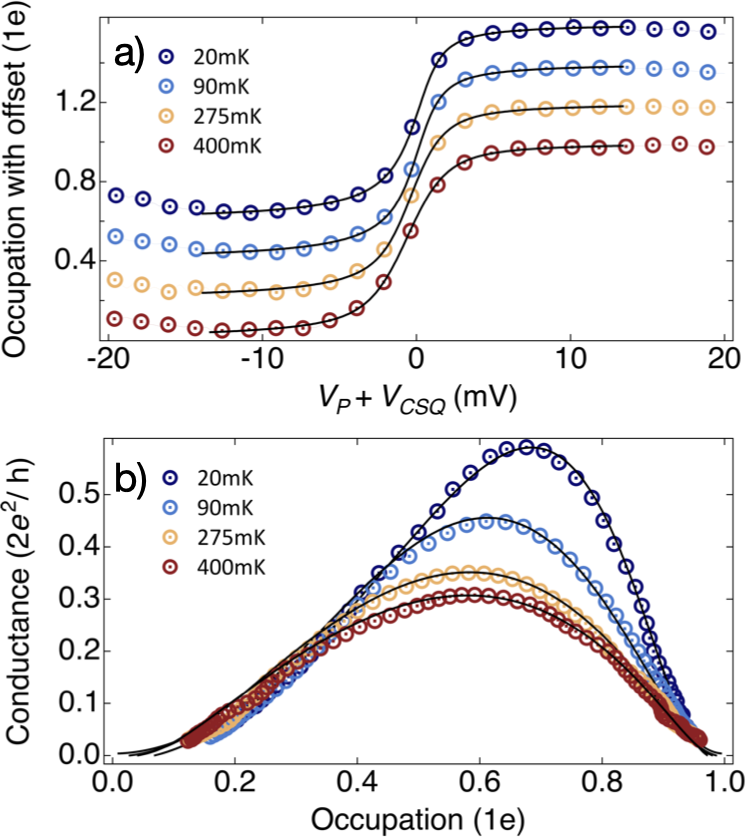
\includegraphics[width=0.8\textwidth]{figures/ch3/crop_FiguresMaster.014.png}
    \caption[Method to determine occupation and plot conductance vs. occupation]{\label{fig:ch3/cond_vs_occ_gf} 
    % For some options that work with pdf\LaTeX, please see this discussion:
    %   \url{http://tex.stackexchange.com/questions/11839}.  
    (\textbf{a}) Charge transitions are converted to occupation by removing the relevant fit parameters. These are amplitude, current offset, cross capacitance of virtual gate and occupation dependant cross capacitance. (\textbf{b}) A plot of conductance vs. occupation is used to show the enhanced conductance due to Kondo. As temperature decreases, the conductance maxima occurs at higher occupation. The NRG (grey) conductance vs. occupation corresponding to the determined $\mathrm{\Gamma/k_BT}$ is plotted ontop of the data where good agreement is found at each temperature.}
  \end{center}
\end{figure}



\begin{figure}[ht]
  \begin{center}
%% includegraphics: comment the following if not using the graphicx package
    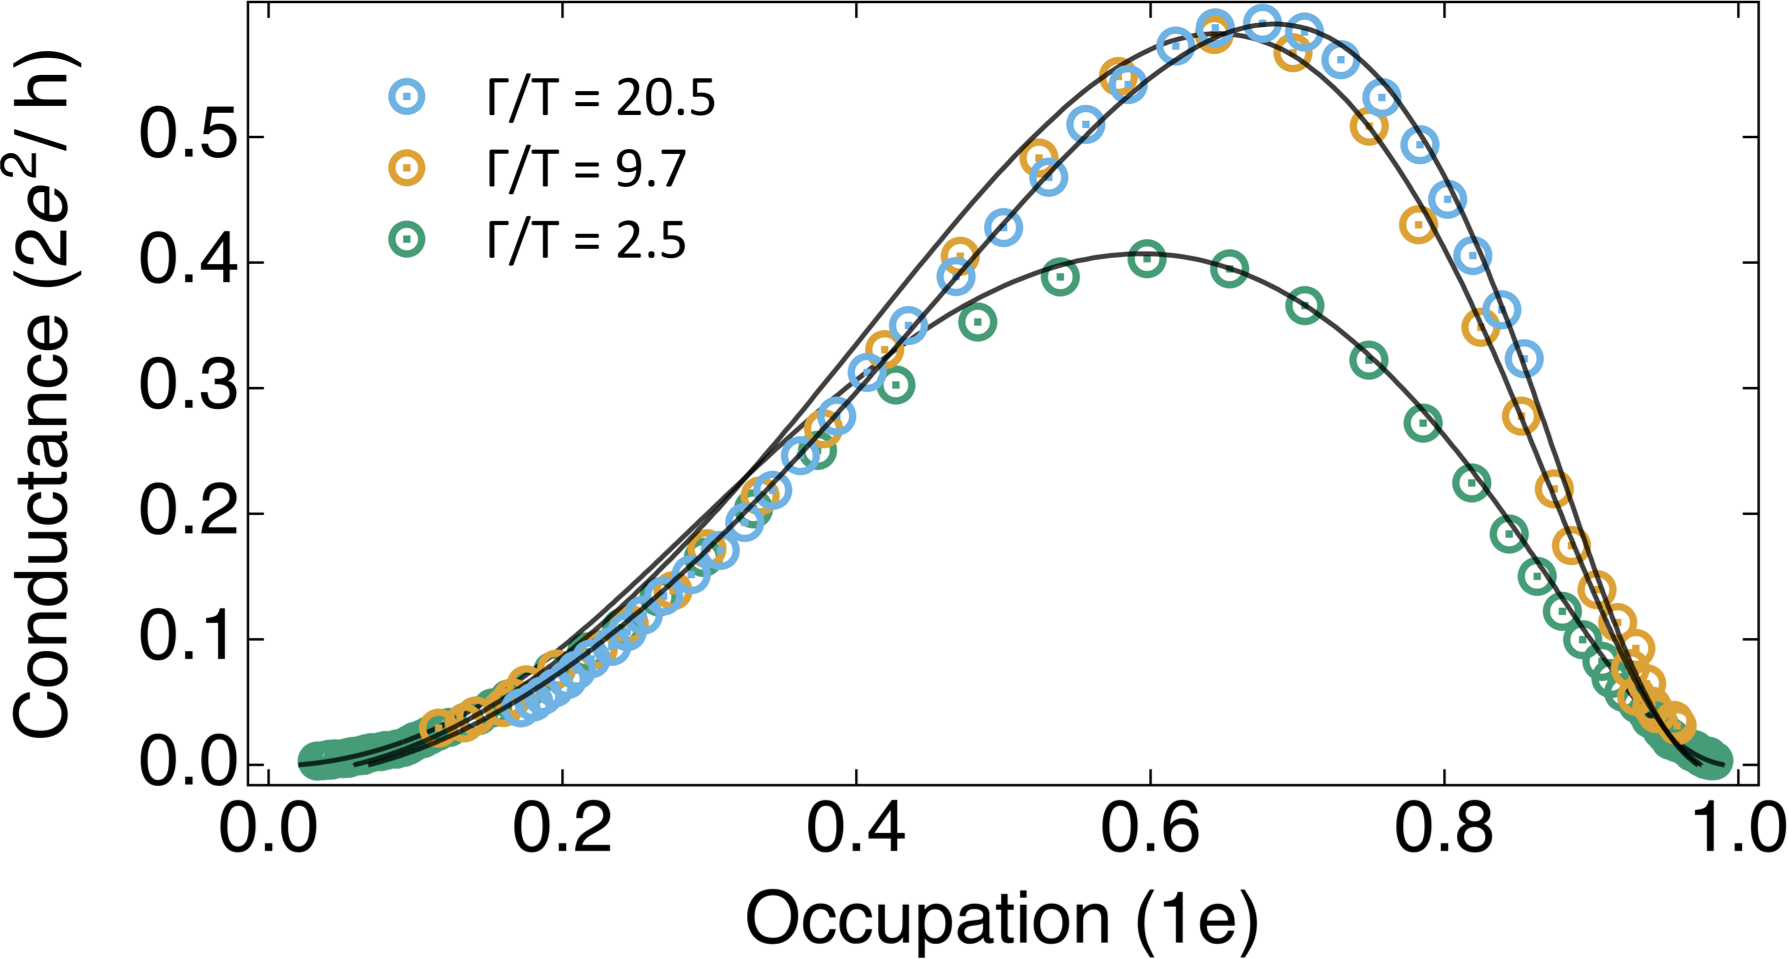
\includegraphics[width=0.8\textwidth]{figures/ch3/crop_FiguresMaster.015.png}
    \caption[Conductance vs. Occupation : Varying the coupling strength between the quantum dot and leads]{\label{fig:ch3/cond_occ_couplingstrength} 
    % For some options that work with pdf\LaTeX, please see this discussion:
    %   \url{http://tex.stackexchange.com/questions/11839}.  
    Conductance vs. occupation in a weak (green) and strong (blue) coupling regime. Each trace is taken at \qty{20}{mK}. The coupling strength $\mathrm{\Gamma/k_BT}$ was determined from a global fit to multiple temperatures. The NRG (grey) conductance vs. occupation corresponding to the determined $\mathrm{\Gamma/k_BT}$ is plotted ontop of the data where good agreement is found at each coupling strength.}
  \end{center}
\end{figure}


\begin{figure}[ht]
  \begin{center}
%% includegraphics: comment the following if not using the graphicx package
    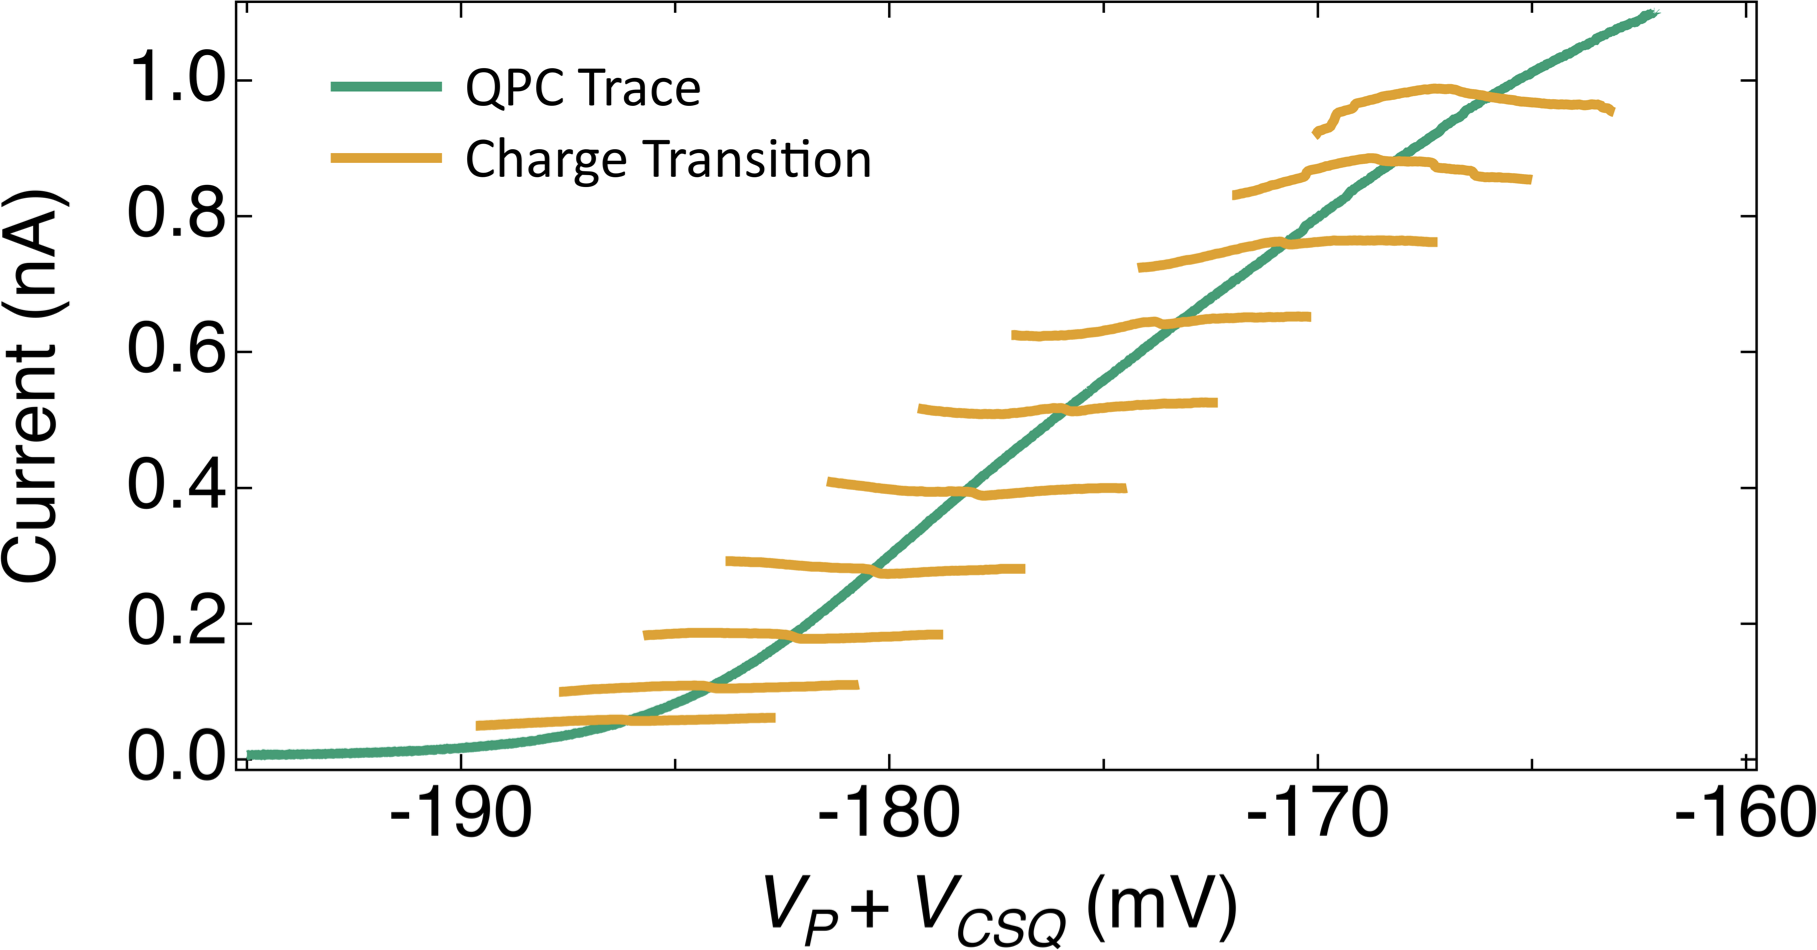
\includegraphics[width=0.8\textwidth]{figures/ch3/crop_FiguresMaster.016.png}
    \caption[Charge transitions measured at various current set points through the charge sensor]{\label{fig:ch3/cond_occ_ct_set-points} 
    % For some options that work with pdf\LaTeX, please see this discussion:
    %   \url{http://tex.stackexchange.com/questions/11839}.  
    Current through the charge sensor (green) from pinch off to the start of the first conductance plateau. Corresponding charge transition (yellow) at each of the current set-points through the charge sensor. Note, the x-axis is not the same between the underlying QPC trace and charge transitions. The charge transitions x-axis has been scaled the same amount for clarity. As the current through the charge sensor is changed, the charge transitions vary dramatically. The left and right slopes curve upwards, downwards, in the same direction or opposite to each other.}
  \end{center}
\end{figure}


\begin{figure}[ht]
  \begin{center}
%% includegraphics: comment the following if not using the graphicx package
    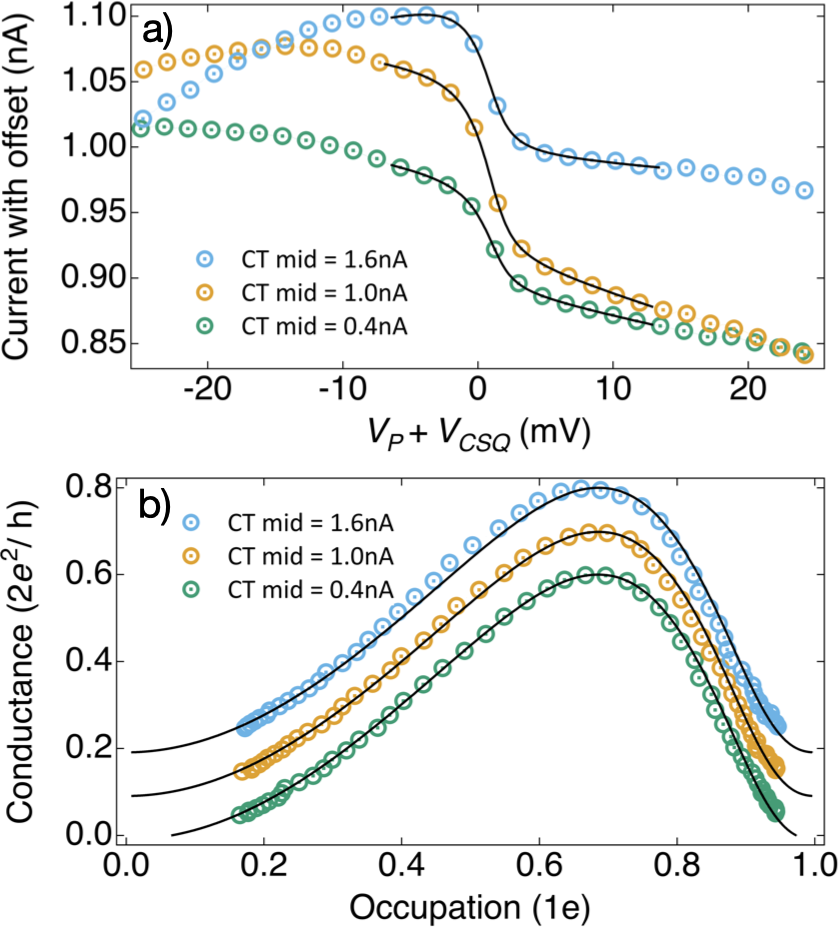
\includegraphics[width=0.8\textwidth]{figures/ch3/crop_FiguresMaster.017.png}
    \caption[Conductance vs. Occupation : Varying the current through the charge sensor]{\label{fig:ch3/cond_occ_QPC_vs_ct} 
    % For some options that work with pdf\LaTeX, please see this discussion:
    %   \url{http://tex.stackexchange.com/questions/11839}.  
    (\textbf{a}) Charge transitions measured with high (blue) and low (green) current through the charge sensor. The transition are offset in current for ease of comparison. The x-axis uses the same virtual gate for each charge transition. The slopes on either side of the charge transitions vary with current through the charge sensor indicating the optimal virtual gate also changes. (\textbf{b}) Conductance vs. occupation ($\mathrm{\Gamma/k_BT=21}$) at different currents through the charge sensor. The traces are offset for clarity. Each trace is taken at \qty{20}{mK}. The coupling strength $\mathrm{\Gamma/k_BT}$ was determined from a global fit to multiple temperatures. The NRG (grey) conductance vs. occupation corresponding to the determined $\mathrm{\Gamma/k_BT}$ is plotted on-top of the data where good agreement is found for each current set-point.}
  \end{center}
\end{figure}



\begin{figure}[ht]
  \begin{center}
%% includegraphics: comment the following if not using the graphicx package
    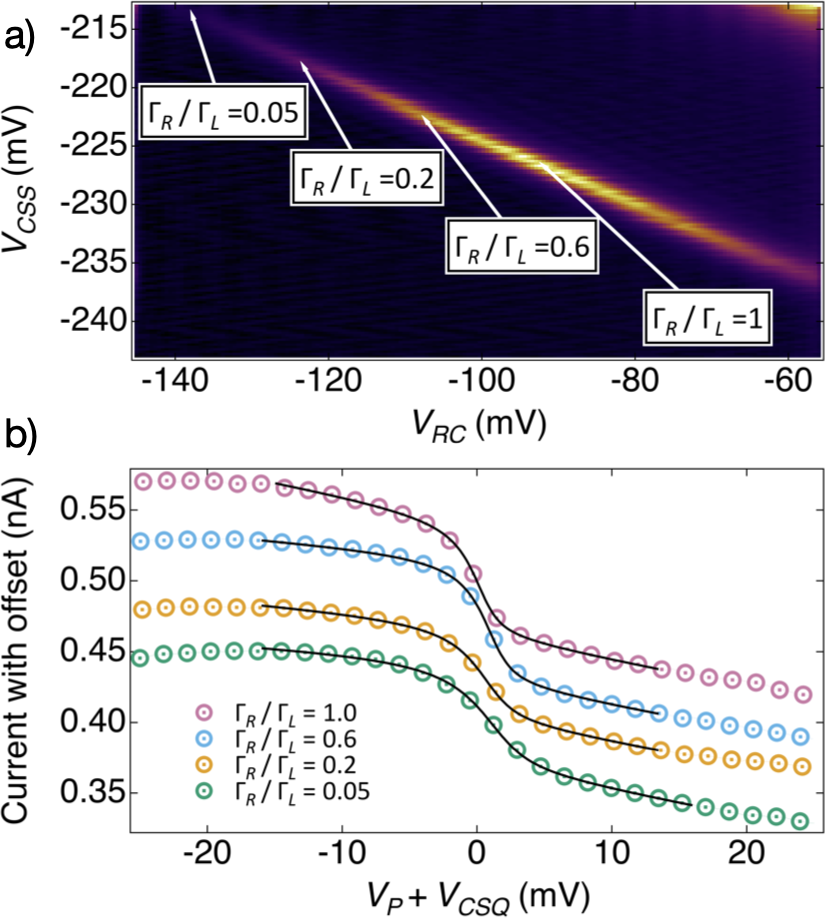
\includegraphics[width=0.8\textwidth]{figures/ch3/crop_FiguresMaster.018.png}
    \caption[Conductance vs. Occupation : Picking locations of varying coupling symmetry]{\label{fig:ch3/symmetry_picking} 
    % For some options that work with pdf\LaTeX, please see this discussion:
    %   \url{http://tex.stackexchange.com/questions/11839}.  
     (\textbf{a}) A 2d scan of conductance through the quantum dot varying the two coupling gates V\textsubscript{CSS} and V\textsubscript{RC}. In the top left, the dot is more coupled to the right reservoir than the left $\mathrm{\Gamma_R} = 0.05\cdot\mathrm{\Gamma_L}$. In the middle of the scan (where the conductance is maximum), the coupling is symmetric $\mathrm{\Gamma_R} = \mathrm{\Gamma_L}$ (\textbf{b}) Charge transitions measured with different ratios of coupling between the two leads in the dot. $\mathrm{\Gamma_R/\Gamma_L} = 1.0$ is symmetric coupling (pink), $\mathrm{\Gamma_R/\Gamma_L} = 0.05$ is asymmetric coupling (green). The transition are offset in current for ease of comparison, but have roughly the same current set-point through the QPC. The x-axis uses the same virtual gate for each charge transition. 
     % The charge transitions become more strongly coupled as asymmetric increases (pink-green)
    }
  \end{center}
\end{figure}


\begin{figure}[ht]
  \begin{center}
%% includegraphics: comment the following if not using the graphicx package
    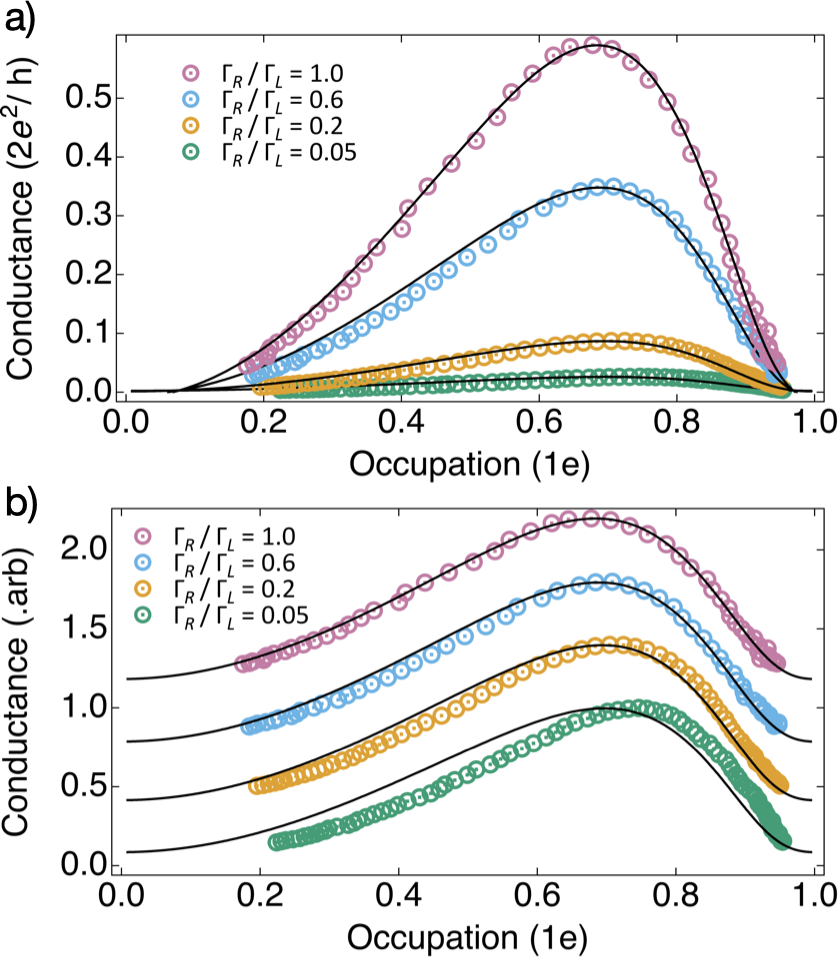
\includegraphics[width=0.8\textwidth]{figures/ch3/crop_FiguresMaster.019.png}
    \caption[Conductance vs. Occupation : Varying the coupling symmetry between quantum dot and leads]{\label{fig:ch3/cond_occ_assymetry} 
    % For some options that work with pdf\LaTeX, please see this discussion:
    %   \url{http://tex.stackexchange.com/questions/11839}.  
    (\textbf{a}) Conductance vs. occupation ($\mathrm{\Gamma/k_BT=21}$) with different ratios of coupling between the two leads in the dot. As the asymmetric is increased, the conductance decreases.
    (\textbf{b}) Same data as in (\textbf{a}), except the traces are offset and scaled for clarity. Symmetric coupling agrees well with NRG calculations, however, the asymmetric coupling data is shifted to the right of predicted NRG. This suggests that $\mathrm{\Gamma/k_BT}$ extracted from the global fit to conductance is lower than expected. }
  \end{center}
\end{figure}